%%%%%%%%%%%%%%%%%%% vorlage.tex %%%%%%%%%%%%%%%%%%%%%%%%%%%%%
%
% LaTeX-Vorlage zur Erstellung von Projekt-Dokumentationen
% im Fachbereich Informatik der Hochschule Trier
%
% Basis: Vorlage svmono des Springer Verlags
%
%%%%%%%%%%%%%%%%%%%%%%%%%%%%%%%%%%%%%%%%%%%%%%%%%%%%%%%%%%%%%

\documentclass[envcountsame,envcountchap, deutsch]{i-studis}

\usepackage{makeidx}         	% Index
\usepackage{multicol}        	% Zweispaltiger Index
%\usepackage[bottom]{footmisc}	% Erzeugung von Fu�noten

%%-----------------------------------------------------
%\newif\ifpdf
%\ifx\pdfoutput\undefined
%\pdffalse
%\else
%\pdfoutput=1
%\pdftrue
%\fi
%%--------------------------------------------------------
%\ifpdf
\usepackage[pdftex]{graphicx}
\usepackage{epstopdf}
\usepackage[pdftex,plainpages=false]{hyperref}
% \usepackage[paper=portrait,pagesize]{typearea}
% \usepackage{rotating}
\usepackage{lscape}
\usepackage{subcaption}
%\else
%\usepackage{graphicx}
%\usepackage[plainpages=false]{hyperref}
%\fi

%%-----------------------------------------------------
\usepackage{color}				% Farbverwaltung
%\usepackage{ngerman} 			% Neue deutsche Rechtsschreibung
\usepackage[english, ngerman]{babel}
%\usepackage[latin1]{inputenc} 	% Erm�glicht Umlaute-Darstellung
\usepackage[utf8]{inputenc}  	% Erm�glicht Umlaute-Darstellung unter Linux (je nach verwendetem Format)

%-----------------------------------------------------
\usepackage{listings} 			% Code-Darstellung
\lstset
{
	basicstyle=\ttfamily, % \scriptsize, 	% print whole listing small
	keywordstyle=\color{blue}, %\bfseries,
								% underlined bold black keywords
	identifierstyle=, 			% nothing happens
	commentstyle=\color{red}, 	% white comments
	stringstyle=\ttfamily, 		% typewriter type for strings
	showstringspaces=false, 	% no special string spaces
	framexleftmargin=7mm, 
	tabsize=3,
	showtabs=false,
	frame=single, 
	rulesepcolor=\color{blue},
	numbers=left,
	linewidth=146mm,
	xleftmargin=8mm,
	language=C++
}
\usepackage{textcomp} 			% Celsius-Darstellung
\usepackage{amssymb,amsfonts,amstext,amsmath}	% Mathematische Symbole
\usepackage[german, ruled, vlined]{algorithm2e}
\usepackage[a4paper]{geometry} % Andere Formatierung
\usepackage{bibgerm}
\usepackage{array}
\usepackage{multicol}

\hyphenation{Ele-men-tar-ob-jek-te  ab-ge-tas-tet Aus-wer-tung House-holder-Matrix Le-ast-Squa-res-Al-go-ri-th-men} 		% Weitere Silbentrennung bei Bedarf angeben
\setlength{\textheight}{1.1\textheight}
\pagestyle{myheadings} 			% Erzeugt selbstdefinierte Kopfzeile
\makeindex 						% Index-Erstellung


%--------------------------------------------------------------------------
\begin{document}
%------------------------- Titelblatt -------------------------------------
\title{Entwicklung eines 2D Charakter-Animationssystemes für automatische Laufbewegungen}
\subtitle{Development of a 2D Character Animation System for Automatic Walking Movements}
%---- Die Art der Dokumentation kann hier ausgew�hlt werden---------------
%\project{Bachelor-Projektarbeit}
\project{Bachelor-Abschlussarbeit}
%\project{Master-Projektstudium}
%\project{Master-Abschlussarbeit}
%\project{Seminar zur Vorlesung ...}
%\project{Hausarbeit zur Vorlesung ...}
%--------------------------------------------------------------------------
\supervisor{Prof. Dr. Christoph Lürig} 		% Betreuer der Arbeit
\author{Daniel Track} 							% Autor der Arbeit
\address{Trier,} 							% Im Zusammenhang mit dem Datum wird hinter dem Ort ein Komma angegeben
\submitdate{20.10.2020} 				% Abgabedatum
%\begingroup
%  \renewcommand{\thepage}{title}
%  \mytitlepage
%  \newpage
%\endgroup
\begingroup
\renewcommand{\thepage}{Titel}
\mytitlepage
\newpage
\endgroup
%--------------------------------------------------------------------------
\frontmatter
%--------------------------------------------------------------------------
% \preface

Ein Vorwort ist nicht unbedingt n�tig. Falls Sie ein Vorwort schreiben, so ist dies der Platz, um z.B. die Firma vorzustellen, in der diese Arbeit entstanden ist, oder einigen Leuten zu danken, die in irgendeiner Form positiv zur Entstehung dieser Arbeit beigetragen haben. Auf keinen Fall sollten Sie im Vorwort die Aufgabenstellung n�her erl�utern oder vertieft auf technische Sachverhalte eingehen.				% Vorwort (optional)
\kurzfassung

%% deutsch
\paragraph*{}
Diese Arbeit beschreibt die Entwicklung eines Systems, das die dynamische Animation der Laufbewegungen von zweidimensionalen Charakteren in Videospielen ermöglicht. Dabei wird zuerst ein Charaktermodell als Skelett erstellt und mit einer Textur versehen. Das Programm erstellt dann anhand der Eingaben des Nutzers und der Daten des Skeletts neue Bewegungsabläufe für jeden einzelnen Schritt des Charakters. Die Bewegungsgeschwindigkeit der so erstellten Animationen sind präzise auf die Eingabe des Spielers abgestimmt und erlaubt Bewegungen über Untergründe verschiedener Höhen.

Dazu werden Hermite Splines für die Hände, Füße und das Becken des Charakters berechnet, denen die entsprechenden Punkte des Körpers dann folgen. Die Splines sind an den Boden unter dem Spieler angepasst und variieren die Schrittweite und -form je nach geforderter Bewegungsgeschwindigkeit.
Außerdem werden die Splines basierend auf einer Reihe von Spline-Prototypen gebildet, die zuvor vom Nutzer festgelegt werden können. So soll eine große Anpassbarkeit der Animationen an verschiedene Charaktere und Anwendungsfälle ermöglicht werden.
Es werden einige Beispiele von Animationen gezeigt, die von dem System erstellt wurden, um die Variation der Bewegungen und den Umgang mit verschiedenen Situationen zu demonstrieren.


%% englisch
\paragraph*{}
This thesis describes the development of a system for the dynamic animation of walking movements for two-dimensional characters in video games. To achieve this, the character model is created as a skeleton and provided with a texture. The application then uses the user's input and the data of the skeleton to generate new animations for every single step of the character. Animations created this way allow for movements with a speed that is fitted precisely to the player's input and that are also able to adapt to differences in ground height.

In order to do this, the system creates Hermite splines for the hands, feet and pelvis of the character that the respective body parts follow. These splines are adjusted to the floor below the player and vary the step distance and shape depending on the required walking speed.
Furthermore, these splines are based on a set of prototype splines that the user may set beforehand. This allows for customization of the created animations in order to fit them to different characters and use cases.
The thesis shows some examples of animations created with the presented system to showcase different possible variations of movements and the adaptation to various situations. 			% Kurzfassung Deutsch/English
\tableofcontents 						% Inhaltsverzeichnis
% \listoffigures 							% Abbildungsverzeichnis (optional)
% \listoftables 							% Tabellenverzeichnis (optional)
%--------------------------------------------------------------------------
\mainmatter                        		% Hauptteil (ab hier arab. Seitenzahlen)
%--------------------------------------------------------------------------
% Die Kapitel werden in separaten .tex-Dateien abgelegt und hier eingebunden.
\chapter{Einleitung}
Diese Arbeit handelt von... (aber ist das genau so wie die Zusammenfassung am Anfang?)

[People are all around us. They inhabit our home, workplace, entertainment, and environment. Their presenceand actions are noted or ignored, enjoyed or disdained, analyzed or prescribed. The very ubiquitousness ofother people in our lives poses a tantalizing challenge to the computational modeler: people are at once themost common object of interest and yet the most structurally complex. from Simulating Humans: Computer Graphics,Animation, and Control]

\section{Motivation}
Obwohl die enorme Leistungsfähigkeit moderner Computer es erlaubt, große, dreidimensionale Welten in Videospielen immer realistischer darstellen zu können, erscheinen noch immer sehr viele zweidimensionale Spiele, die das große Potenzial dieser Maschinen nicht ausreizen. Dafür mag es eine Reihe von Gründen geben, angefangen bei der Nostalgie vieler Spieler für die 2D-Spiele älterer Konsolengenerationen bis hin zu den meist wesentlich komplexeren mathematischen Verfahren, die zur Programmierung von dreidimensionalen Anwendungen verwendet werden. In vielen Fällen wird es jedoch auch damit zu tun haben, dass die Erstellung von 3D-Modellen und deren Animation besonders kleine Entwicklerstudios vor eine große Herausforderung stellt. 2D-Assets hingegen können recht leicht mit einem der vielen verfügbaren Bildbearbeitungsprogramme erstellt oder sogar per Hand gezeichnet und digitalisiert werden.

Einen entscheidenden Vorteil bieten 3D-Modelle jedoch gegenüber 2D-Sprites: Zur Animation werden 3D-Objekte meist auf ein Skelett gespannt, für dessen Knochen dann Zielstellungen angegeben werden. Das Modell folgt dann der Bewegung der Knochen. Bei 2D-Modellen hingegen wird häufig jeder einzelne Schritt der Animation zuvor erstellt. Auch hier gibt es Verfahren, mit denen Computer den Grafikdesignern Arbeit abnehmen können; trotzdem wird meist eine beachtliche Anzahl an Animationsframes per Hand erstellt. Viele der 2D-Spiele sind deshalb außerdem auf eine Framerate von 60 Bildern pro Sekunde limitiert. Monitore mit höheren Framerates werden aber zunehmend günstiger und populärer, und 120, 144 oder gar 240 FPS zu unterstützen stellt für die gängigen 2D-Animationssysteme eine schwierige Herausforderung dar, während es bei den meisten 3D-Anwendungen hauptsächlich eine Frage der Hardware ist.

Ein weiterer Vorteil der gängigen 3D-Animationsverfahren ist, dass genaue Zielpunkte für Bewegungen während der Laufzeit des Programms errechnet und Animationen dann so ausgeführt werden können, dass sie diese Punkte exakt treffen (z.B. wenn ein Charakter ein Objekte mit seiner Hand greift). Mit 2D-Animationen, deren Bilder vor der Laufzeit des Programms gezeichnet werden, ist dies nicht möglich.

Eine Übertragung des Verfahrens der skelettbasierten Animation auf 2D-Charaktere könnte dabei helfen, sowohl den Arbeitsaufwand bei der Erstellung von Animationen zu minimieren als auch neue Arten von Animationen zu ermöglichen, die erst zur Laufzeit des Programms gebildet werden.

\section{Zielsetzung}
Um die Vorteile der zuvor beschriebenen skelettbasierten Animierung von 2D-Charakteren zu demonstrieren, soll ein System erstellt werden, dass nur einen einzelnen Sprite eines Charakters verwendet und eine Laufanimation darstellt. Um weiterhin zu zeigen, welche Möglichkeiten das Einbeziehen von Laufzeitdaten eröffnet, soll der Charakter auch über Flächen verschiedener Höhen (wie z.B. eine Treppe hinauf) laufen können und dabei sowohl die Position, auf der der Fuß aufgesetzt wird als auch die Bewegung dorthin dynamisch zur Laufzeit errechnen.

Eine wichtige Limitierung dabei ist, dass ausdrücklich \textit{nicht} Ziel dieser Arbeit ist, physikalisch korrekte Bewegungen zu zeigen. Auf den Charakter wirkt also keine Gravitation, er muss kein Gleichgewicht halten oder sein Momentum abbremsen. Die Bewegung soll jedoch glaubhaft aussehen, kann dabei aber durchaus stilisiert sein, wie es in der Computeranimation üblich ist.

\section{Aufbau}
\chapter{Forschungsstand} \label{forschungsstand}
Das folgende Kapitel gibt einen Überblick über bestehende Literatur, die für das hier vorgestellte Animationssystem relevant ist. Zuerst werden dabei die Arbeiten zu prozeduralen Animationssystemen vorgestellt. Da sich die meisten dieser Beiträge mit Bewegungen im dreidimensionalen Raum beschäftigen, können ihre Ergebnisse häufig leider nur beschränkt auf diese Arbeit übertragen werden. Im zweiten Teil wird dann der Forschungsstand zur skelettbasierten Animation von zweidimensionalen Objekten erläutert. Zuletzt wird beschrieben, wie sich die hier vorliegende Arbeit in den Kontext der bestehenden Forschung einfügt und welchen Beitrag sie leisten soll.


\section{Prozedurale Laufanimation}
Da Laufbewegungen einen der wohl häufigsten Bewegungsabläufe von Menschen darstellen, gibt es eine lange Reihen von Arbeiten zum Problem der Animation von menschlichen Laufbewegungen. In vielen Fällen werden die beschriebenen Animationen dabei einmalig erstellt und dann genau so abgespielt und aufgezeichnet (beispielsweise für computergenerierte Charaktere in einem Film). Da Videospiele ein interaktives Medium sind, ist es zur Anwendung in Spielen jedoch oft wichtig, dass die Animationen noch zur Laufzeit des Programms an das gewünschte Verhalten angepasst werden können. Ansätze zur Erstellung von Bewegungen zur Laufzeit können grob in drei Kategorien unterteilt werden: Prozedurale Bewegung (auch algorithmische Bewegung), beispielbasierte Bewegung und dynamisch-simulierte Bewegung \cite{johansen2009automated}.

Systeme zur prozeduralen Bewegung verwenden ein Verständnis für die Bewegungsabläufe von Charakteren, um neue Bewegungen spontan generieren zu können. Beispielbasierte Ansätze hingegen schöpfen aus einer Reihe von zuvor erstellten Animationen und kombinieren diese, um neue Bewegungsabläufe zu erstellen. Bisweilen kommen dabei auch noch prozedurale Techniken zum Einsatz, um die kombinierten Animationen weiter an die benötigte Situation anzupassen. Dynamische Simulationen hingegen berechnen ein physikalisches Modell des Charakters und seiner Umgebung und versuchen so, realistische Bewegungen zu erstellen. Als Grundlage können dabei auch Beispielanimationen oder prozedural erstellte Bewegungen verwendet werden.

Einen Ansatz zur prozeduralen Generierung von Laufbewegungen in Echtzeit beschreiben Bruderlin und Calvert\cite{bruderlin1993interactive}\cite{bruderlin1996knowledge}. Sie simulierten die grundlegende Bewegung der Beine als wären sie ein umgekehrtes Pendel und approximierten die Flugbahn des Torsos in der Luft mit einer Parabel. Ihr System bietet dem Nutzer eine große Anzahl von Variablen zur Beeinflussung der Animation und ermöglicht so viele verschiedene, ausdrucksstarke Bewegungen, trotz ihrer rein synthetischen Natur. Es sind aber nur Bewegungen auf ebenen Untergründen möglich.

Ein weiteres Team um Bruderlin\cite{bruderlin1994procedural} entwickelte das \textit{Life Forms} System zur Animation von menschlichen Figuren im dreidimensionalen Raum. Sie verwendeten dabei Inverse Kinematics, um die Figuren mit ihren Händen nach Objekten greifen zu lassen. Die Bewegungen der anderen daran beteiligten Körperteile wie Arm und Schulter wurden dabei durch die Knochen und die für diese zuvor festgelegten Beschränkungen errechnet. Außerdem bietet ihre Anwendung die Möglichkeit zur prozeduralen Erstellung von Laufbewegungen. Dabei werden als Hauptparameter die Schrittweite und Schrittfrequenz (und daraus resultierend die Laufgeschwindigkeit) vom Nutzer angegeben. Das Programm erstellt dann vier Kontrollpunkte für einen Schritt in der Laufbewegung: Den Anfang, das Ende und dazwischen die beiden Zeitpunkte, an denen die Hüfte am höchsten bzw. am niedrigsten ist. Daraufhin wird eine kubische Spline-Kurve berechnet, die durch diese vier Punkte verläuft. Die Position der Hüfte des Modells wird dann entlang dieser Kurve interpoliert und die Stellung der Beine dazu passend berechnet.

Dem Problem des unebenen Terrains widmeten sich Chung und Kollegen\cite{chung1999animation}. Die von ihnen entwickelten Algorithmen ermöglichen die automatische Bewegung über Untergründe verschiedener Höhe, während die verwendete Collision Detection dafür sorgt, dass die Beine dabei nicht durch Hindernisse bewegt werden. Außerdem gibt es ein hierarchisches System von Stellschrauben, die zur Justierung der Animation genutzt werden können.

Johansen\cite{johansen2009automated} entwickelte ein System zur Fortbewegungsanimation von 3D-Charakteren, das prozedurale Verfahren mit beispielbasierten Ansätzen verbindet. Er nutzte dabei nur zwei verschiedene Beispielanimationen -- bei einer läuft der Charakter geradeaus, bei der anderen bewegt er sich zur Seite -- unter der Annahme, dass sich aus diesen beiden Bewegungen alle anderen synthetisieren lassen würden. Die Resultate dieses Schritts werden dann prozedural mittels Inverse Kinematics an die Höhe und den Winkel des Untergrunds angepasst, sodass der Charakter auch über Stufen oder schräge Flächen laufen kann. Die Ergebnisse dieses Systems wirken dabei durchweg glaubhaft.

Auf dieser Arbeit aufbauend versuchte Shapiro\cite{shapiro2011building}, variablere, ausdrucksstärkere Animationen mit einem ähnlichen Funktionsspektrum zu erreichen. Er stellte dem System mit 19 Exemplaren eine größere Menge an Beispielanimationen zur Verfügung, um den prozeduralen Bestandteil und Inverse Kinematics aus dem Verfahren entfernen zu können (und trotzdem noch alle verschiedenen Bewegungsmöglichkeiten abzudecken). Er beschreibt die Resultate seiner Arbeit als realistischer, die Erstellung der vielen Beispielanimationen sorgt aber für einen wesentlich größeren Aufwand, wenn das System in Projekten verwendet werden soll.

\section{Skelettbasierte Animation von 2D-Objekten}
Einen der frühen Versuche, skelettbasierte Animation für die Bewegungen zweidimensionaler Charaktere zu verwenden, stellten Burtnyk und Wein\cite{burtnyk1976interactive} vor. Bis dahin wurden häufig Keyframes von Animationen gezeichnet und die restlichen Bilder durch Interpolation dieser Keyframes erzeugt. Dieses System erlaubte jedoch nur geradlinige Bewegung in gleich großen Schritten zwischen den Keyframes. Die Autoren führten ein Skelett in das Animationssystem ein, welches es erlaubte, mit verhältnismäßig wenig Aufwand eine hohe Anzahl von Keyframes zu erstellen, da nur die simple Strichmännchen-Repräsentation dieses Skeletts neu gezeichnet werden musste. Das finale Bild wird dann anhand des Skeletts in entsprechende Posen verzerrt.

Van Overveld\cite{van1990technique} beschrieb ein Verfahren zur 2D-Animation, bei dem das Skelett vom Rest des Objekts getrennt wurde. Das Skelett bzw. einige seiner Punkte wurden dann prozedural in Echtzeit animiert und die Bewegungen der restlichen Punkte dynamisch simuliert. Die beschränkenden Kräfte auf das Skelett wurden bei dieser Simulation erst nur approximiert und später dann korrigiert, um eine Performance zu erreichen, die schnell genug für eine Darstellung in Echtzeit ist.

Auf diesem Artikel aufbauend entwickelten Aoki et al.\cite{aoki1999dynamic} ein Verfahren zur realistischen Animation von Pflanzen, die vom Wind bewegt werden. Sie verwendeten dazu digital erstellte Bilder von Pflanzen und versahen sie per Hand mit Skeletten. Diesen Skeletten wurden dann mechanische Eigenschaften zugewiesen, mit denen die Simulation im letzten Schritt arbeitete. Sie beschreiben ihre Ergebnisse als sehr realistisch, mehr als zwei im Artikel enthaltene Beispielbilder konnten aber nicht gefunden werden, um das zu bestätigen.

Ein noch nicht lange zurückliegendes Paper von Pangesti und Kollegen\cite{pangesti2019analysis} beschreibt die Entwicklung eines Verfahrens zur einfacheren Erstellung von Laufanimationen für 2D-Charaktere mithilfe eines Skeletts und Inverse Kinematics. Außerdem war ein weiteres erklärtes Ziel ihrer Arbeit, eine Animation für das Umkehren während des Laufens zu erzeugen. Durch die Analyse von Laufbewegungen echter Menschen bestimmten sie die Freiheitsgrade der verschiedenen Knochen und wendeten diese auf das virtuelle Skelett an. So wird automatisiert verhindert, dass beispielsweise ein Ellenbogen in die falsche Richtung geknickt wird. Ein Animator kann dann Keyframes festlegen, denen der Körper des Modells folgen soll, ohne dass dadurch Fehlstellungen entstehen können. Die Arbeit demonstriert dieses Verfahren zuletzt dann noch mit einer Animation für das Umkehren des Charakters während der Laufbewegung. Bemerkenswert dabei ist, dass das verwendete Modell dreidimensional ist und dann gerendert wird, um die Frames für die finale, zweidimensionale Animation zu erzeugen.


\section{Einordnung in die bestehende Literatur}
Um die Animationen des Charakters präzise an die Gegebenheiten des Untergrunds anzupassen, auf dem der Charakter sich bewegt, ist entweder ein (teilweiser) prozeduraler Ansatz oder eine dynamische Simulation vonnöten. Da dynamische Simulationen aufgrund ihrer physikalischen Modelle meist einen höheren Rechenaufwand mit sich bringen und außerdem primär realistische Bewegungsabläufe generieren können (was nicht Ziel dieser Arbeit ist -- die Bewegungen sollen nur glaubhaft aussehen), werden diese Ansätze hier nicht weiter verfolgt. Ideen der beispielbasierten Animation, speziell die Interpolation zwischen mehreren zuvor erstellten Bewegungsabläufen, könnten dabei helfen, Laufbewegungen individueller und ausdrucksstärker erscheinen zu lassen und außerdem die Komplexität des prozeduralen Systems durch ihre Bewegungsvorgaben reduzieren.

Die hier beschriebenen Beiträge zur skelettbasierten Animation von 2D-Charakteren hatten meist nicht zum Ziel, in interaktiven Systemen verwendet zu werden. Sie sollten vielmehr Animatoren als Werkzeug zu dienen, welches den Animationsprozess vereinfacht. Das in dieser Arbeit vorgestellte System soll speziell für die Anwendung in Videospielen erstellt werden. Dass die generierten Animationen durch die Eingaben des Spielers maßgeblich beeinflusst werden bedeutet dabei auch, dass die Designer nicht die Möglichkeit haben, Animationen per Hand zu korrigieren, bevor der Spieler sie zu Gesicht bekommt. Somit sollte möglichst gewährleistet werden, dass die Animationen ein vorhersagbares Verhalten zeigen. Sie sollen sich also an die Eingaben des Spielers anpassen, dabei aber nicht zu grob von der vom Animator geplanten Bewegung abweichen.

Außerdem soll durch das Erstellen und darauf folgende Animieren eines einzelnen 2D-Sprites der Designaufwand minimiert werden. Pangesti et al.\cite{pangesti2019analysis} verwendeten zwar skelettbasierte Verfahren, um 2D-Animationen zu erstellen, der dem zugrunde liegende Charakter ist aber ein dreidimensionales Modell, was sowohl die Erstellung des Modells als auch das Animationssystem wesentlich komplizierter macht. Einen der großen Vorteile dabei demonstrierten sie aber auch in ihrer Arbeit: Es kann eine Animation für das Umkehren des Charakters erstellt werden, bei der die Körperteile sich realistisch verdecken. Diese Möglichkeit fällt bei der Verwendung von Sprites weg, da das System keine Informationen über die Tiefenverhältnisse der Körperteile hat. Demnach stellt dies eine Limitierung des hier präsentierten Systems dar.

Da die Idee dieser Arbeit darauf basiert, Techniken aus der 3D-Charakteranimation auf 2D-Charaktere zu übertragen, können auch einige der Erkenntnisse aus der Forschung zur Bewegungsanimation in 3D übertragen werden. Dazu zählen unter anderem Collision Detection wie bei Chung et al.\cite{chung1999animation} oder die Kombination von prozeduraler Planung der Schritte mit vorgefertigten Beispielanimationen, wie sie von Johansen\cite{johansen2009automated} demonstriert wurde.
\chapter{Grundlagen}

\section{Skelettbasierte Animation}

\section{Hermitekurven}
\chapter{Implementierung} \label{implementierung}
Nachdem in den vorherigen Kapiteln theoretische Vorarbeit geleistet wurde, soll nun die Implementierung des geplanten Animationssystems erläutert werden. Begonnen wird dabei mit der konzeptionellen Planung der Software. Da diverse Bibliotheken zur Vereinfachung der Programmierarbeit verwendet wurden, werden diese dann kurz beschrieben. Als nächstes folgt eine visuelle und schriftliche Darstellung des Programmaufbaus, bevor dann der Animationsprozess detailliert erklärt wird.


\section{Konzeption}
Da der hauptsächliche Anwendungsbereich des in dieser Arbeit beschriebenen Animationssystems Videospiele sind, werden zur Implementierung auch Werkzeuge verwendet, die in der Spieleindustrie gängig sind. Programmiert wird deshalb in C++ unter Windows und mit einem x64-Prozessor als Zielplattform. Um eine gute Performance des Programms zu gewährleisten, soll ein möglichst großer Teil der Berechnungen auf der Grafikkarte ausgeführt werden. Dafür kommt OpenGL als Grafikbibliothek zum Einsatz und es werden Shader in GLSL geschrieben.

Um das Ziel der präzisen Bestimmbarkeit der Bewegungsgeschwindigkeit zu erreichen, wird davon ausgegangen, dass die Simulation mit einem Gamepad gesteuert wird. Die Laufgeschwindigkeit soll dann aus den Eingabedaten des Control Sticks errechnet werden.

Außerdem soll zur Synthese von Animationen für die verschiedenen Laufgeschwindigkeiten ein Verfahren zum Einsatz kommen, das aus zwei zuvor festgelegten Animationen eine neue erstellt, die auf die geforderte Situation passt (angelehnt an das Verfahren von \cite{johansen2009automated}).

Um flüssige Bewegungen der Gliedmaßen zwischen vorbestimmten Punkten in der Simulation möglich zu machen, sollen Hermite Splines generiert werden, die die entsprechenden Punkte verbinden. Daraufhin sollen Inverse Kinematics angewendet werden, um die Gliedmaßen entlang der Splines zu bewegen.

\section{Verwendete Bibliotheken}
Um viele der grundlegenden Prozesse im Programm zu vereinfachen und schon gut gelöste Probleme wie z.B. das Erstellen eines OpenGL-Kontexts oder das Laden der Modelldaten nicht erneut lösen zu müssen, werden einige Bibliotheken verwendet. Diese werden im Folgenden im Detail erläutert.

\subsection{OpenGL}
\href{https://www.opengl.org/}{OpenGL} ist eins der meist verwendeten Grafik-APIs und bietet als solches diverse Funktionen, um mit der Grafikkarte zu interagieren. Es bietet außerdem die Shading-Language GLSL, die zur Programmierung der Shader verwendet wird. In dieser Anwendung kommt die Version 3.3 Core zum Einsatz.

\subsection{OpenGL Mathematics (GLM)}
Bei \href{https://glm.g-truc.net/0.9.9/index.html}{GLM} handelt es sich um eine Mathematik-Bibliothek für C++, die der Namensgebung und Funktionalität von GLSL entspricht und deren Datenformate so aufgebaut sind, dass sie den von GLSL erwarteten Formaten entsprechen. Die von GLM bereitgestellten Matrix- und Vektorklassen und die Funktionen, die mit ihnen arbeiten, werden für Berechnungen auf der CPU sowie zum Hochladen von Daten in den GPU-Speicher verwendet.

\subsection{Simple DirectMedia Layer (SDL)}
\href{https://www.libsdl.org/index.php}{SDL} ist eine leichtgewichtige C-Bibliothek, die das Erstellen und Verwalten eines Fensters und des dazugehörigen OpenGL-Kontexts unter Windows stark vereinfacht. Außerdem bietet sie mit simplen Funktionen Zugang zu Maus-, Tastatur- und Gamepad-Inputs. Des Weiteren wird die dazugehörige Bibliothek \href{https://www.libsdl.org/projects/SDL_image/}{SDL\_image} zum Laden von Bildern im PNG-Format verwendet.

\subsection{Open Asset Import Library (Assimp)}
Das Skelett des zu animierenden Charakters und damit zusammenhängend auch das Mesh sowie die UV-Koordinaten und Bone-Weights liegen dem Programm im FBX-Format vor. \href{http://assimp.org/}{Assimp} ermöglicht es, dieses Dateiformat zu parsen und dabei einige Post-Processing Operationen wie das Vereinigen identischer Vertices durchzuführen.

\subsection{Dear ImGui}
Bei \href{https://github.com/ocornut/imgui}{Dear ImGui} handelt es sich um eine Implementierung des Immediate Mode GUI Paradigmas. Es ermöglicht die Darstellung von grafischen Interfaces im bestehenden OpenGL-Kontext und wird hier verwendet um Debug-Informationen anzuzeigen, die erstellten Tools zu kontrollieren und einige Variablen der Simulation zur Laufzeit ändern zu können.

\section{Aufbau des Programms} \label{aufbau}
Das UML-Klassendiagramm in Abb. \ref{uml_classes} zeigt den generellen Aufbau der Anwendung. Im Zentrum steht dabei die Klasse \lstinline{Game}, die auf hoher Ebene den Ablauf koordiniert und die verschiedenen Komponenten der Simulation verwaltet. Ihre Methode \lstinline{init()} initialisiert alle nötigen Systeme und erstellt das Fenster, sodass das Programm in einem geeigneten Ausgangszustand ist. Die Methode \lstinline{run()} berechnet den nächsten Simulationsschritt und zeichnet das Ergebnis auf den Bildschirm.

Zum Zeichnen der Grafiken und Verwalten der Shader wird \lstinline{Renderer} verwendet. Er lädt bei seiner Initialisierung die vier verschiedenen Shader-Programme, die in der Anwendung zum Einsatz kommen und besitzt jeweils ein Objekt der vier entsprechenden Shader-Klassen \lstinline{DebugShader}, \lstinline{TexturedShader}, \lstinline{RiggedShader} und \lstinline{BoneShader}. Die verschiedenen Shader und ihre Anwendungsgebiete werden in Abschnitt \ref{rendering_section} ausführlicher beschrieben.

Die Klassen \lstinline {MouseKeyboardInput} und \lstinline{Gamepad} verwalten die verschiedenen Eingabemöglichkeiten und werden zu Beginn jedes Frames aktualisiert. Bei der Klasse \lstinline{Background} handelt es sich um eine sehr einfache Klasse, die nur dafür zuständig ist, eine Textur als Hintergrund zu rendern. Der Hintergrund stellt einen Referenzpunkt für die Bewegungen des Charakters dar und erleichtert so die Beurteilung der Animationen.

\lstset{keywordstyle=\color{black}} % so the word default in default.level is not blue
Da der Charakter über Untergründe verschiedener Höhen laufen können soll, wurde die Klasse \lstinline{Level} zur Repräsentation der Bodenstruktur erstellt. Der Untergrund besteht dabei aus einer Reihe von Collidern, die jeweils aus Quadraten bestehen und entlang der globalen X- und Y-Achsen ausgerichtet sind. Um den Aufbau des Levels anzupassen, gibt es außerdem den \lstinline{LevelEditor}. Er bietet ein simples User Interface zum Erstellen, Löschen und Verändern der Levelelemente. Weiterhin besteht die Möglichkeit, die Level in einem selbst erstellten Dateiformat zu speichern und wieder zu laden. Beim Start des Programms wird immer die Datei \lstinline{assets/default.level} geladen, über den Editor können aber auch noch weitere Levels zum Testen verschiedener Aspekte der Simulation geladen werden.
\lstset{keywordstyle=\color{blue}}

\lstinline{Player} repräsentiert den Spielercharakter und ist eine Unterklasse von \lstinline{Entity}. Er besitzt ein \lstinline{Mesh}, das wiederum aus einer Reihe von Vertices und Knochen besteht. Zusammen mit der Textur bietet es die Grundlage für die visuelle Darstellung des Charakters. Kontrolliert wird letzterer hauptsächlich mit den Inputdaten des \lstinline{Gamepad}.

Der \lstinline{Animator} steuert die Bewegungen des Spielercharakters und bildet somit den Kern der Anwendung. Er beinhaltet Repräsentationen der vier Gliedmaßen des Spielers in \lstinline{limbs} und eine Sammlung von Spline-Prototypen, an denen die Bewegungsabläufe orientiert werden, in \lstinline{spline_prototypes}. Der genaue Ablauf des Animationsprozesses wird in Abschnitt \ref{animator_section} ausführlich erklärt.


\subsection{Rendering und Shader} \label{rendering_section}
Alle Klassen, die grafische Objekte in der Simulation darstellen, haben eine Methode \lstinline{void render(const Renderer&)} (eventuell noch mit weiteren Parametern), mit der sie sich selbst auf den Bildschirm zeichnen. Die Objekte wählen dann einen der vier verschiedenen Shader aus, indem sie auf dem entsprechenden Member-Objekt des Renderers \lstinline{use()} aufrufen und setzen gegebenenfalls noch Uniform-Variablen. Die zu rendernden Vertexdaten halten die Objekte in einer Instanziierung des Templates \lstinline{VertexArray<>} mit dem zum Shader passenden Vertextyp als Template-Argument. Sie rufen auf diesem VertexArray \lstinline{draw(GLenum mode)} auf, um die Vertices im entsprechenden Modus zeichnen zu lassen. Die vier verfügbaren Shader sind:
\begin{enumerate}
    \item \lstinline{DebugShader}
    \item \lstinline{TexturedShader}
    \item \lstinline{RiggedShader}
    \item \lstinline{BoneShader}
\end{enumerate}

Der \lstinline{DebugShader} wird hauptsächlich zur Visualisierung von Debug-In\-for\-ma\-tio\-nen verwendet. Es kann eine Farbe für die zu rendernden Primitive in Form einer Uniform-Variable eingestellt werden; Texturen werden nicht verwendet. Das Vertexformat dieses Shaders besteht nur aus einem zweidimensionalen Vektor zur Angabe der Vertexposition. Außerdem gibt es die statische Variable \lstinline{DEFAULT_VAO}, die ein simples Vertex Array zur Darstellung von quadratischen Objekten anbietet. Diese müssen so nicht ihre eigenen Vertices im Arbeitsspeicher der GPU verwalten, sondern können die beschriebenen Vertices verwenden und mithilfe der Model-Matrix beliebig transformieren.

Bei texturierten Objekten kommt der \lstinline{TexturedShader} zum Einsatz. Seine Vertices enthalten deshalb neben der Position noch eine Texturkoordinate; er funktioniert ansonsten aber sehr ähnlich wie der \lstinline{DebugShader}.

Der \lstinline{RiggedShader} wird immer dann verwendet, wenn ein animierter Charakter mit Skelett gerendert werden soll. Er ist der komplexeste der hier verwendeten Shader und transformiert die Vertices anhand der ihnen zugeordneten Knochen. Seine Input-Vertices bestehen deshalb aus vier Komponenten: Neben Position und Texturkoordinate noch die Indizes der zwei Knochen, die diesen Vertex beeinflussen, und die dazugehörigen Gewichtungen. Die Transformationsmatrizen der verschiedenen Knochen werden vor dem Rendering auf der CPU berechnet und als Uniform-Variable auf die GPU hochgeladen, wo der Shader dann auf sie zugreifen kann.

Der \lstinline{BoneShader} zeichnet die Knochen des Modells. Seine Input-Vertices sollten jeweils Head- und Tail-Position der Knochen des Modells sein. Die Vertices sollten in der gleichen Reihenfolge wie die Knochen des Modells vorliegen, denn der Shader verwendet die gleichen Bone-Transformationsmatrizen wie der \lstinline{RiggedShader} und berechnet den Index des zu verwendenden Knochens aus dem Index des Vertices (geteilt durch Zwei). So können die Vertices wie beim \lstinline{DebugShader} lediglich aus einem zweidimensionalen Vektor zur Angabe der Position bestehen.

Nur die Klassen \lstinline{Mesh}, \lstinline{Background} und \lstinline{Spline} verwenden eigene Vertex-Arrays auf der GPU. Nur \lstinline{Spline} verändert diese Daten nach der Initialisierung, die anderen beiden transformieren die Vertices nur noch durch Uniforms.

\section{Animationsprozess} \label{animator_section}
Zur Animation des Charakters bestimmt der \lstinline{Player} in seiner Update-Methode zunächst die aktuelle Bewegungsgeschwindigkeit anhand der Eingaben des Spielers. Sollte der Charakter gerade in die entgegengesetzte Richtung der Eingabe blicken, wird außerdem das Modell entlang der Y-Achse gespiegelt. Daraufhin ruft der \lstinline{Player} die Update-Methode des \lstinline{Animator}s auf und gibt dabei die Bewegungsgeschwindigkeit -- zusammen mit einer Liste der Collider im Level und dem Faktor \lstinline{delta_time}, der die vergangene Zeit seit dem letzten Simulationsschritt angibt -- als Argumente weiter.

Ein Aktivitätsdiagramm der nun folgenden Abläufe zur Animation des Charakters ist in Abb. \ref{uml_activity} zu sehen. Der \lstinline{Animator} bestimmt zunächst anhand der Bewegungsgeschwindigkeit und des aktuellen Animationszustands, ob eine neue Animation bestimmt werden muss. Ist dies der Fall, wird der neue Animationszustand in \lstinline{leg_state} gespeichert und die Methode \lstinline{set_new_splines} aufgerufen, die daraufhin die nächste Animation berechnet.

Als nächstes wird der Interpolationsfaktor der Animation abhängig von dem Zeitfaktor \lstinline{delta_time} erhöht und die Rotation des Rückens weiter zu ihrer Zielrotation hin interpoliert. Zuletzt berechnet das Programm anhand des Interpolationsfaktors und der jeweiligen Splines die aktuellen Zielpunkte für die Gliedmaßen und sucht mittels Inverse Kinematics nach einer passenden Stellung für die beiden Gelenke des Arms oder Beins. Damit endet die Update-Methode des \lstinline{Animator}s und der \lstinline{Player} verschiebt seine Position zur neuen Beckenposition.

\subsection{Generierung neuer Animationen}
Für die Erstellung neuer Animationen sorgt die Methode \lstinline{set_new_splines}. Sie bestimmt als erstes anhand der Laufgeschwindigkeit eine Zielrotation für den Rücken des Charakters. Diese dient dazu, dass letzterer sich beim Rennen in die Bewegungsrichtung lehnt. Um flüssige Bewegungsabläufe zu gewährleisten wird dieser Wert nicht direkt als Rotation des entsprechenden Knochens gesetzt, sondern lediglich als Zielwert, zu dem der Knochen dann hin interpoliert.

Daraufhin wird zwischen zwei verschiedenen Fällen unterschieden, die unterschiedliche Animationen erfordern: Entweder der Charakter steht still, oder er bewegt sich. Da die Animation für den stehenden Charakter (Idle-Animation) aus einer leichten auf und ab Bewegung besteht, muss hier zuerst festgestellt werden, in welche Richtung die Animation als nächstes ausgeführt werden soll. Daraufhin werden für die Arme die entsprechenden Spline-Prototypen ausgewählt und an die richtige Position relativ zum Arm transformiert. Außerdem wird der Startpunkt der Spline an die aktuelle Position der Hand gesetzt. Dieser Schritt findet in fast allen Fällen beim setzen eines neuen Splines für Gliedmaßen statt und gewährleistet, dass es keine Sprünge in der Animation gibt. Stattdessen sollen immer weiche Bewegungen von einem Punkt zum nächsten erfolgen.

Für die Beine wird bei der Idle-Animation nach dem Boden direkt unter dem Hüftknochen gesucht und ein Spline direkt von der aktuellen Position des Fußes dort hin verwendet. Das Becken verwendet als Basis seiner Bewegung wie die Arme einen Spline-Prototypen. Da der ganze Körper des Charakters der Bewegung des Beckens folgt, muss beim Erstellen eines Splines sichergestellt werden, dass die Beine immer den Boden erreichen können. Der Richtwert für die Höhe des Beckens über dem Boden wird durch eine Membervariable in \lstinline{Animator} vorgegeben, deren Wert immer kleiner oder gleich groß sein sollte wie die Länge eines Beins. Als Boden unter dem Becken wird außerdem immer der niedrige der beiden Untergründe unter den Beinen gewählt. Zuletzt wird der so ermittelte Spline dann je nach aktueller Richtung der Idle-Animation noch umgedreht.

Steht der Spieler hingegen nicht still, wird zunächst anhand der gewünschten Bewegungsgeschwindigkeit die Länge des nächsten Schritts ermittelt. Sollte der Charakter gerade erst los laufen, wird diese Schrittweite halbiert, um die Position für den vorderen Fuß nicht so weit nach vorne zu setzen, dass das Bein diese gar nicht mehr erreichen kann. Im Folgenden wird dann zur Bestimmung der Splines für die verschiedenen Gliedmaßen jeweils zwischen zwei Spline-Prototypen für Gehen und Rennen interpoliert. Der dabei verwendete Interpolationsfaktor ist wie die Schrittweite von der Laufgeschwindigkeit abhängig.

Die Splines für die Arme werden durch die gerade beschriebene Interpolation berechnet und der Zielpunkt um eine Schrittweite in Bewegungsrichtung verschoben. Letzteres ist nötig, um die Position des Punkts relativ zum Körper konstant zu halten, da die Splines in Weltkoordinaten angegeben werden und der Körper des Charakters sich bis zu Ende des Schritts um eben diese Schrittweite bewegt haben wird.

Die beiden Beine führen beim Laufen jeweils verschiedene Bewegungen aus und müssen deshalb getrennt betrachtet werden. Das führende Bein berechnet zunächst die Interpolation der beiden Spline-Prototypen, passt dann aber noch sowohl den Ausgangs- als auch den Endpunkt an. Als Ausgangspunkt wird die aktuelle Fußposition gesetzt. Der Fuß soll sich am Ende des Schritts eine halbe Schrittweite vor dem Körper befinden, deshalb wird als X-Koordinate des Endpunkts die des Ausgangspunkts verwendet und um 1,5 Schrittweiten nach vorne verschoben. Das Level wird an dieser Stelle nach geeignetem Untergrund durchsucht und die Höhe von diesem als Y-Koordinate verwendet. Bei diesem Verfahren werden zwar die beiden interpolierten Punkte vollständig missachtet, die Interpolation hat aber trotzdem einen Zweck, da die so bestimmten Tangenten den Stil der Bewegung maßgeblich bestimmen.

Da andere Bein steht während des gesamten Schritts am gleichen Ort auf dem Boden; sein Spline ist deshalb trivial bestimmbar: Beide Punkte entsprechen der aktuellen Fußposition, beide Tangenten haben die Länge Null.\footnote{Eigentlich könnte diese Position auch einfach direkt festgelegt und gar kein Spline mehr verwendet werden. Es müsste dann aber ein Sonderfall für das stehende Bein im Code eingeführt werden, der das System zwar möglicherweise effizienter, dafür aber auch schwieriger verständlich machen würde.}

Zuletzt wird dann noch die Bewegung des Beckens bestimmt. Dazu werden wieder die interpolierten Spline-Prototypen genutzt, die Startposition auf die aktuelle Beckenposition gesetzt und die X-Koordinate der Zielposition als eine Schrittweite davon entfernt festgelegt. Zur Bestimmung der Y-Koordinate berechnet das Programm die durchschnittliche Höhe der beiden Beine und fügt dem Ergebnis die im \lstinline{Animator} eingestellte Beckenhöhe hinzu. Als letztes wird dann noch der Faktor zur Interpolation auf den Splines auf Null zurückgesetzt, sodass alle Animationen bei ihrem Startpunkt beginnen.

\begin{landscape}
    \begin{figure}
        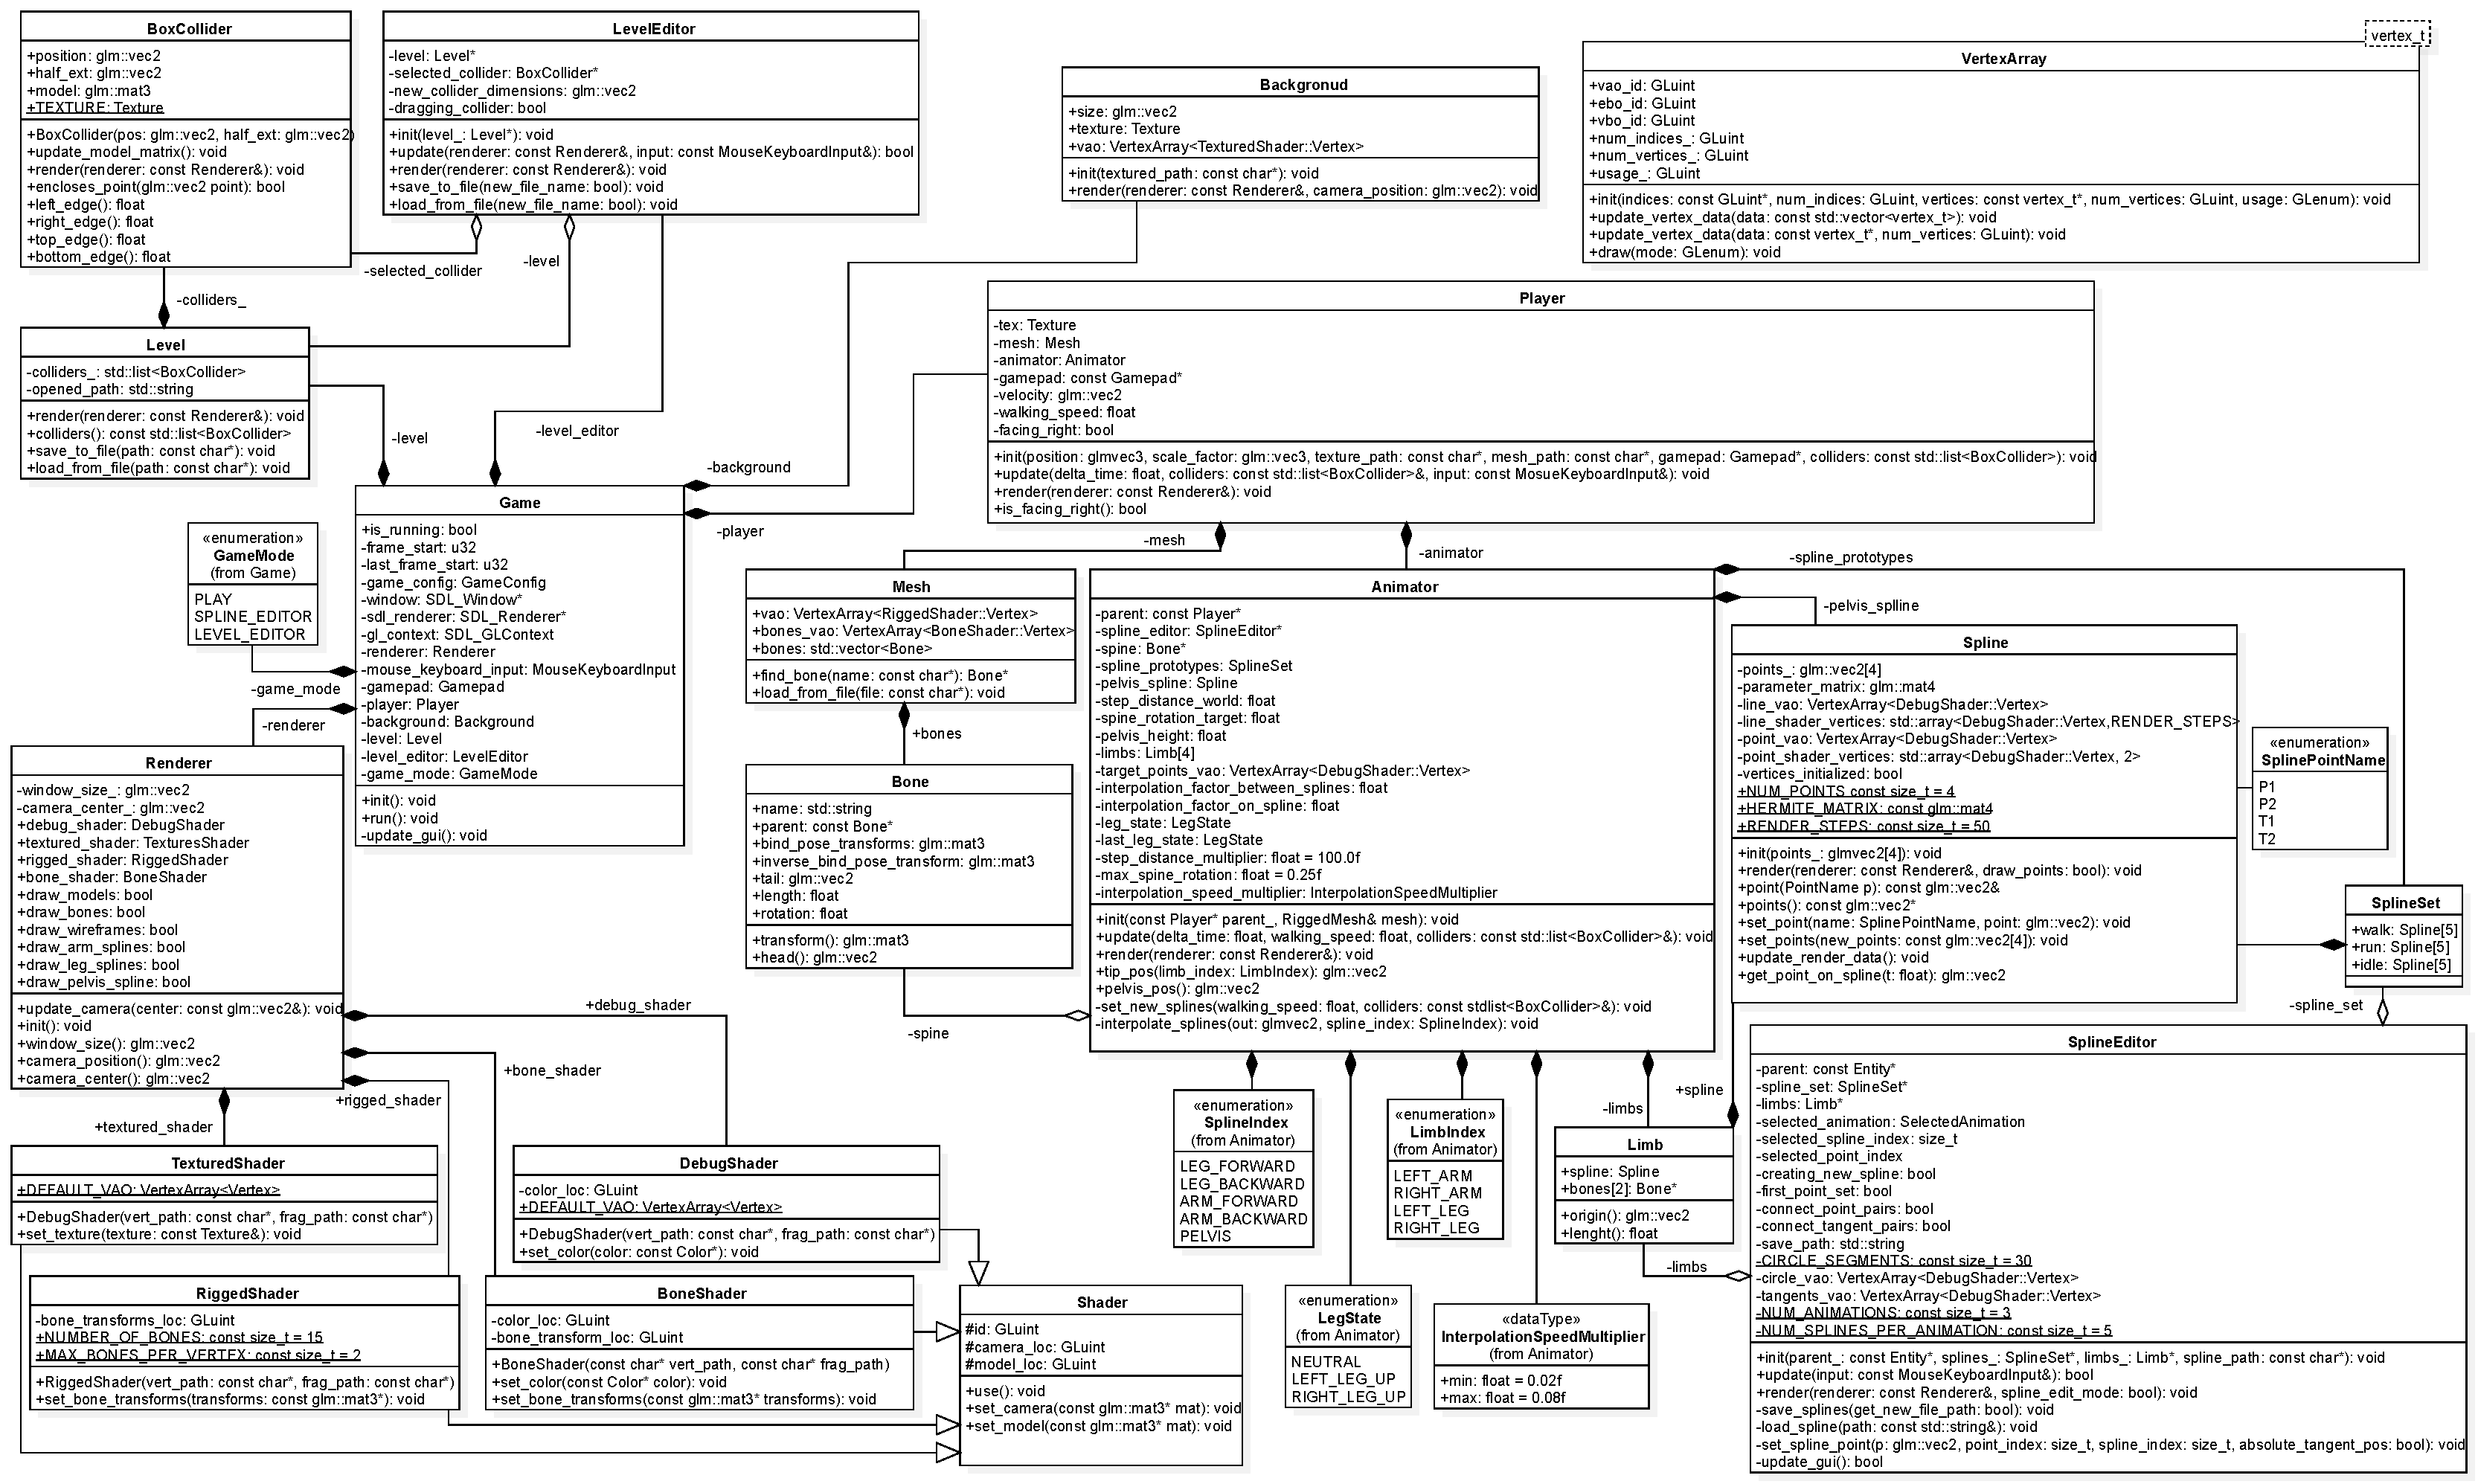
\includegraphics[width=\linewidth]{images/ClassDiagram.pdf}
        \caption{Objektdiagramm des gesamten Programms. Einige Klassen und Assoziationen wurden zur Verbesserung der Übersichtlichkeit ausgelassen.}
        \label{uml_classes}
    \end{figure}
\end{landscape}

\begin{figure}
    \centering
    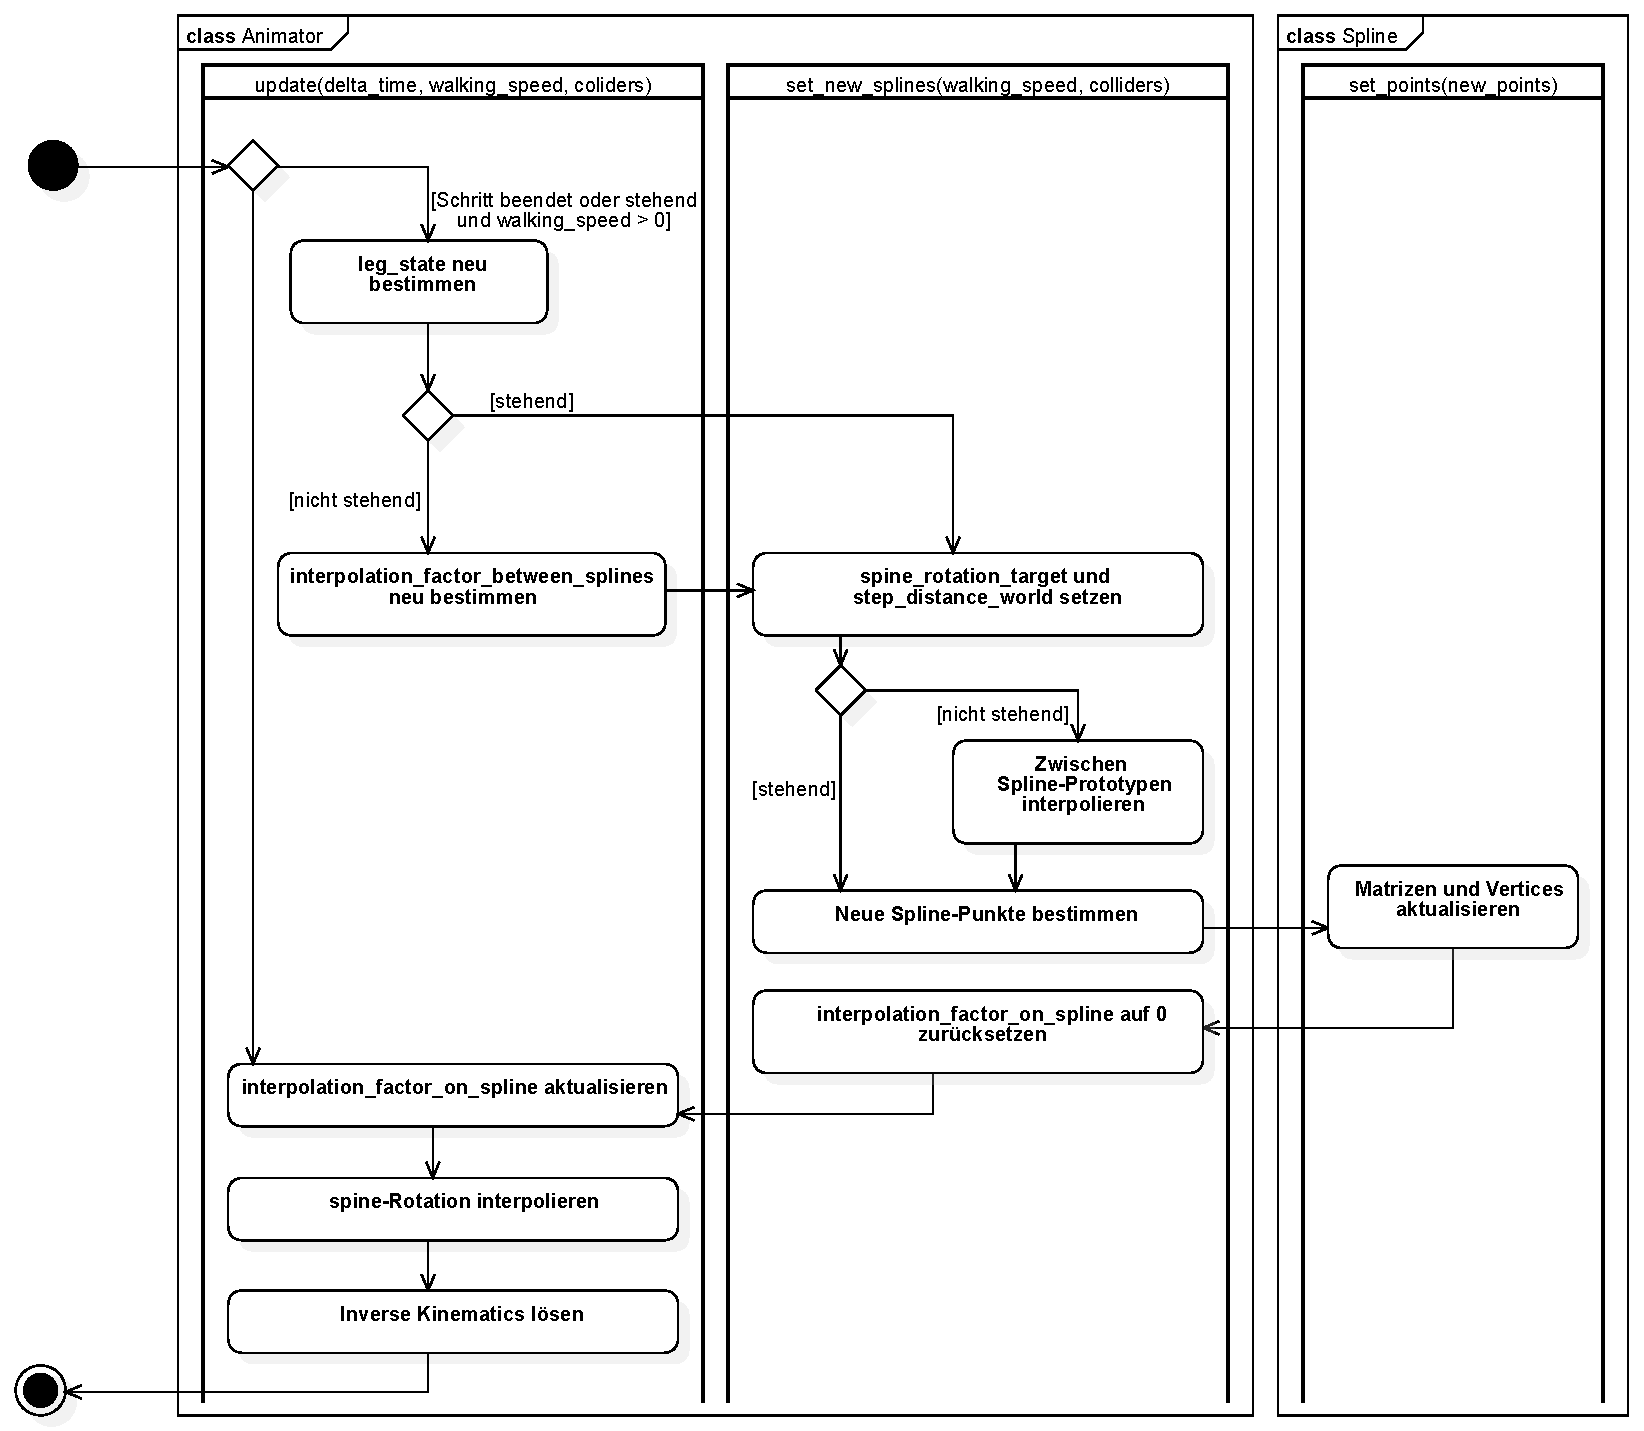
\includegraphics[width=\linewidth]{images/AnimatorActivity.pdf}
    \caption{Aktivitätsdiagramm des Animationsprozesses}
    \label{uml_activity}
\end{figure}

\subsection{Anpassung der Bewegungen}
Um den Stil der generierten Animationen an die Persönlichkeit des animierten Charakters anzupassen, erlaubt das Interface direkten Zugriff auf die Membervariablen \lstinline{step_distance_multiplier}, \lstinline{interpolation_speed_multiplier} und \lstinline{max_spine_rotation} des \lstinline{Animator}s. Außerdem wurde ein Editor für die Spline-Prototypen implementiert, der direkt mit den Daten \lstinline{Animator}s arbeitet und diese auch in einem Binärformat speichern und laden kann.
\chapter{Ergebnisse}
Allgemein kann festgestellt werden, dass das Versuch, die hauptsächlich in der der 3D-Animation verwendete Technik der skelettbasierten Animation zur dynamischen Animation von 2D-Charakteren zu Nutzen, erfolgreich war. Das entwickelte System verwendet ein Skelett und erstellt anhand einiger zuvor festgelegter Splines für jeden Schritt eine neue Bewegungsabfolge. Wird ein Mesh erstellt und den einzelnen Vertices Knochen zugeteilt, werden die Vertices und die darauf gezeichnete Textur anhand des Skeletts verformt.

Der Charakter verfügt dabei über die Möglichkeit, anhand der Auslenkung des Control-Sicks präzise seine Schrittweite und Bewegungsgeschwindigkeit anzupassen. Beispiele für eine langsame und eine schnelle Bewegungsanimation sind in Abb. \ref{even_slow} bzw. Abb. \ref{even_fast} zu sehen. Die Interpolation zwischen zwei verschiedenen Splines -- einem für das langsame Gehen, einem für das Rennen -- sorgt dabei dafür, dass nicht nur die Länge des Schritts wächst, sondern auch die Form der Bewegung sich verändert.

Des Weiteren wurde das Ziel erreicht, Bewegungen über Flächen verschiedene Höhen möglich zu machen. Der Charakter sucht sich dabei an der gewünschten nächsten Fußposition den passenden Boden und berechnet einen Spline mit dem entsprechenden Punkt als Ziel. Eine Animation für das Hinaufsteigen einer Stufe wird in Abb. \ref{uphill} gezeigt, das Hinabsteigen einer solchen ist in Abb. \ref{downhill} zu sehen. Eine entscheidende Limitierung ist dabei aber, dass gerade bei kleinen Schritten mangels Collision Detection für die Splines nicht sichergestellt werden kann, dass die dynamisch erstellten Bewegungen nicht mit dem Level kollidieren, wie in Abb. \ref{clip_through_ground} gezeigt.

Um dem Ziel der Responsivität gerecht zu werden, ist es dem Charakter möglich, auch mitten in einem Schritt abrupt stehen zu bleiben. Da ein solches plötzliches Stoppen in der Realität jedoch nicht ohne Weiteres möglich ist, könnte dies zu einer unglaubwürdigen Animation führen könnte. Um mit diesem Problem umzugehen wird die Bewegung des Charakters zwar sofort gestoppt, es wird aber eine Übergangsanimation eingefügt, um die Abruptheit etwas zu verschleiern. Zum stehen kommen kann der Charakter dabei auch auf unebenem Untergrund und bewegt sich dabei stets so, dass seine Beine sauber auf dem Boden stehen (siehe Abb. \ref{standing_uneven}).\footnote{Ein angemessenes Level wird dabei vorausgesetzt. Sind die Unterschiede zwischen benachbarten Untergründen zu groß, um realistisch auf ihnen stehen zu können, entstehen fehlerhafte Animationen.}

Außerdem werden diverse Möglichkeiten geboten, die Generierung der Animationen anzupassen. Durch die Veränderung von Schrittweite, dem Grad des Einlehnens in die Bewegungsrichtung und der Geschwindigkeit der Interpolation auf den errechneten Splines sind bereits einige Stellschrauben gegeben. Weiterhin wird aber auch noch der Spline-Editor angeboten, der die präzise Anpassung der einzelnen Splines ermöglicht, die wiederum die Grundlage der dynamisch gebildeten Animationen darstellen. Die Kombination dieser Anpassungsmöglichkeiten erlaubt dem Nutzer, eine Vielzahl von verschiedenen Bewegungsmustern für die zu animierenden Charaktere zu erstellen.

% \section{Limitierungen}

\begin{figure}
    \centering
    \begin{subfigure}[t]{.4\linewidth}
        \centering
        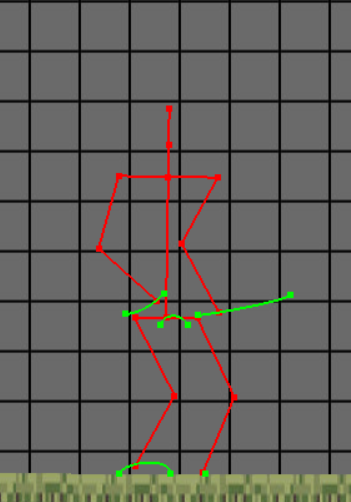
\includegraphics[width=0.75\linewidth]{images/even_ground_slow.png}
        \caption{Gehen auf ebenem Untergrund.}
        \label{even_slow}
    \end{subfigure}
    \begin{subfigure}[t]{.4\linewidth}
        \centering
        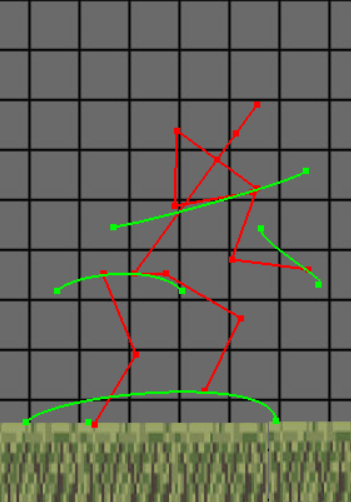
\includegraphics[width=0.75\linewidth]{images/even_ground_fast2.png}
        \caption{Rennen auf ebenem Untergrund.}
        \label{even_fast}
    \end{subfigure}
    \begin{subfigure}[t]{.4\linewidth}
        \centering
        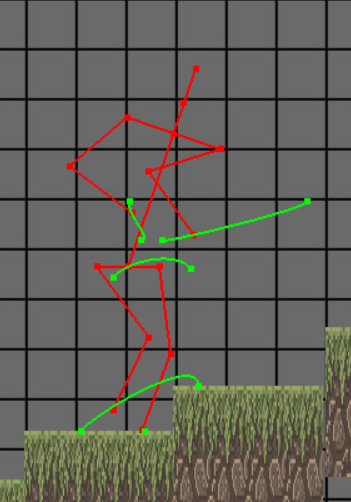
\includegraphics[width=0.75\linewidth]{images/going_up3.png}
        \caption{Bewegung bergauf.}
        \label{uphill}
    \end{subfigure}
    \begin{subfigure}[t]{.4\linewidth}
        \centering
        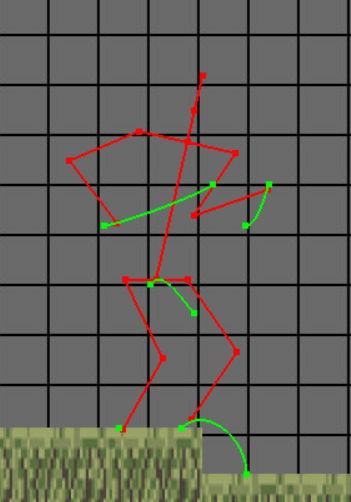
\includegraphics[width=0.75\linewidth]{images/going_down1.png}
        \caption{Bewegung bergab.}
        \label{downhill}
    \end{subfigure}
    \begin{subfigure}[t]{.4\linewidth}
        \centering
        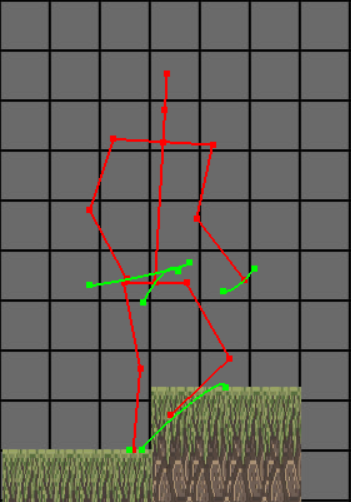
\includegraphics[width=0.75\linewidth]{images/clip_through_gorund.png}
        \caption{Ein Bein bewegt sich beim aufwärts gehen durch den Boden.}
        \label{clip_through_ground}
    \end{subfigure}
    \begin{subfigure}[t]{.4\linewidth}
        \centering
        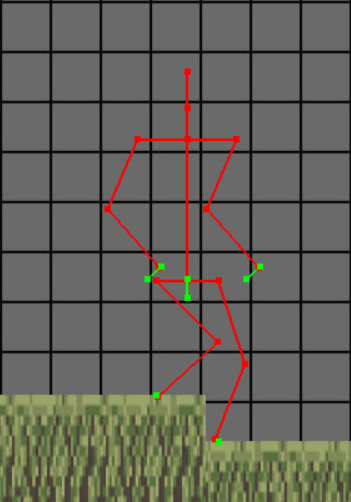
\includegraphics[width=0.75\linewidth]{images/standing_uneven.png}
        \caption{Stehen auf unebenem Untergrund.}
        \label{standing_uneven}
    \end{subfigure}
    \caption{Beispiele generierter Animationen. Das Skelett ist in rot dargestellt. Die grünen Linien stellen die Splines dar, an denen sich die entsprechenden Knochen entlang bewegen.}
\end{figure}
\chapter{Zusammenfassung und Ausblick}
In dieser Arbeit wurde versucht, ein System zu entwickeln, das die automatische Laufanimation von zweidimensionalen Charakteren zur Laufzeit des Programms anhand eines Skeletts und eines einzelnen Sprites ermöglicht. Dieses Ziel wurde erreicht; der Charakter kann sich dabei auch über verschieden hohe Untergründe und in beliebiger Geschwindigkeit bewegen. Außerdem reagiert der Charakter dabei meist schnell auf Eingaben und der Rechenaufwand der Simulation ist überschaubar, was die Verwendung in einem Videospiel begünstigt. Ein Editor für die zur Animation verwendeten Splines ermöglicht die Anpassung der Bewegungsabläufe an die Bedürfnisse des Nutzers.

Das System verfügt jedoch auch noch über viele Limitierungen, an denen zukünftige Arbeiten ansetzen könnten. Beispielsweise ist aktuell immer ein Fuß fest an den Boden gebunden, obwohl Menschen beim Rennen in der Regel zeitweise keinen Kontakt mehr zum Bode haben. Ein offensichtlichen Fehler ist außerdem die fehlende Collision Detection beim Bewegen über unebenen Untergrund. So kann es häufig vorkommen, dass sich beispielsweise der Fuß des Charakters durch ein Hindernis bewegt. Durch die Verwendung passender Splines lässt sich das Problem etwas minimieren, was aber die Anpassungsmöglichkeiten der Animation stark einschränkt.

Im Zusammenhang mit dieser Problematik der Kollisionsvermeidung wäre es möglicherweise hilfreich, eine komplexere Art von Splines zu verwenden. Die aktuellen Hermite Splines bestehen immer nur aus zwei Punkten und den zwei dazugehörigen Tangenten, ein dritter Punkt könnte jedoch beispielsweise an den Mittelpunkt des Schritts gesetzt werden, um die Bewegung besser zu definieren und um Hindernisse herum zu navigieren. Ein komplexeres System zur Anpassung der Tangenten in diesem dritten Punkt wäre dann aber vermutlich auch vonnöten, um bei Schritten auf höhere oder niedrigere Ebenen einen gutaussehenden Bewegungsablauf zu wahren.

Außerdem funktioniert der Algorithmus zum Finden der neuen Fußpositionen nur mit Collidern, die entlang der X- und Y-Achsen der Spielwelt ausgerichtet sind. Schräge Flächen sind also nicht möglich. Hier könnte das System leicht erweitert werden, um mehr Variation in den Levels zu erlauben.




% In diesem Kapitel soll die Arbeit noch einmal kurz zusammengefasst werden. Insbesondere sollen die wesentlichen Ergebnisse Ihrer Arbeit herausgehoben werden. Erfahrungen, die z.B. Benutzer mit der Mensch-Maschine-Schnittstelle gemacht haben oder Ergebnisse von Leistungsmessungen sollen an dieser Stelle pr�sentiert werden. Sie k�nnen in diesem Kapitel auch die Ergebnisse oder das Arbeitsumfeld Ihrer Arbeit kritisch bewerten. W�nschenswerte Erweiterungen sollen als Hinweise auf weiterf�hrende Arbeiten erw�hnt werden.



% Limits:
% - kein flight-state beim rennen
% - keine physikalische simulation
% - keine verlangsamung/beschleunigung bei bergauf/bergab gehen
% - kein kopf bone, ist aber evtl unnötig

% - shape deformation des charakters kann hart sein, kein fancy algorithmus dafür wird angewendet
% > wäre aber auch cpu/gpu intensiv, also für spiele lieber nicht? würde zumindest viel optimierungsarbeit kosten
% % - keine schrägen oberflächen, collision detection nur aabb
% - keine foot-base
% - zyklische bewegungen
% - nur humanoide, könnte aber erweitert werden
% % - collision derection nicht trivial, bei IK sogar extra hart wenn man alles auf einmal beachten will (also z.B. knie in den boden bei laufen)
% - umkehren sieht kacke aus, keine umkehranimation

% - bleibt der charakter stehen, sieht die aimation etwas komsich aus. dafür mehr responsive als wenn er zurück oder weiter steppen würde
% - je nachdem wann input gepollt wird kann erster schritt oft sehr klein sein

% Verbesserungen:
% - punkte festlegen, durch die die splines verlaufen sollen (siehe bruderlin1994procedural)
% - mehrere schritte in die zukunft simulieren, um besser auf hindernisse reagieren zu können (siehe Animation of Human Walking in Virtual Environments)
% ...
%--------------------------------------------------------------------------
\backmatter                        		% Anhang
%-------------------------------------------------------------------------
\bibliographystyle{geralpha}			% Literaturverzeichnis
\bibliography{literatur}     			% BibTeX-File literatur.bib
%--------------------------------------------------------------------------
\printindex 							% Index (optional)
%--------------------------------------------------------------------------
\begin{appendix}						% Anh�nge sind i.d.R. optional
    % \chapter{Glossar}

\abbreviation{DisASTer}		{DisASTer (Distributed Algorithms Simulation Terrain), A platform for the Implementation of Distributed Algorithms}
\abbreviation{DSM}			{Distributed Shared Memory}
\abbreviation{AC}			{Linearisierbarkeit (atomic consistency)}
\abbreviation{SC}			{Sequentielle Konsistenz (sequential consistency)}
\abbreviation{WC}			{Schwache Konsistenz (weak consistency)}
\abbreviation{RC}			{Freigabekonsistenz (release consistency)}
			% Glossar   
    \chapter{Erkl�rung der Kandidatin / des Kandidaten}

\begin{description}[$\Box$~]
\item[$\Box$] Die Arbeit habe ich selbstst�ndig verfasst und keine anderen als die angegebenen Quellen und Hilfsmittel verwendet.\\

\item[$\Box$] Die Arbeit wurde als Gruppenarbeit angefertigt. Meine eigene Leistung ist\\
...\\

Diesen Teil habe ich selbstst�ndig verfasst und keine anderen als die angegebenen Quellen und Hilfsmittel verwendet. \\

Namen der Mitverfasser: ...

\end{description}

\vspace{2cm}

\begin{minipage}[t]{3cm}
\rule{3cm}{0.5pt}
Datum
\end{minipage}
\hfill
\begin{minipage}[t]{9cm}
\rule{9cm}{0.5pt}
Unterschrift der Kandidatin / des Kandidaten
\end{minipage}	% Selbstst�ndigkeitserkl�rung
\end{appendix}

\end{document}
